% =====================================================================
%  c07：原印刷页 55–63（PDF p.56–64）
%  §2.2.12、§2.2.13、§2.2.14、§2.2.15
%  （四个标题均为 \subsubsection，其父 \section 属第 2 章，已由前序片段定义）
%  公式编号 (2.224)–(2.265) 连续；含原文 Figure 5、Figure 6。
%  本片段不含 \section 级标题，故按规范不插入 keytakeaways。
% =====================================================================

\medskip
\noindent\textbf{评注}：\emph{非交换环面代数}。设 $\Lambda$ 是带整值辛形式的格（integral symplectic lattice）。非交换环面代数（noncommutative torus algebra），又称无理旋转代数（irrational rotation algebra），是由满足下式的酉算子 $X_\gamma$ 生成的 $C^*$-代数：

\begin{equation}
  X_{\gamma_1}X_{\gamma_2}=q^{\langle\gamma_1,\gamma_2\rangle}X_{\gamma_1+\gamma_2}
  \tag{2.224}
  \label{eq:2.224}
\end{equation}

其中 $q$ 是某个复数。这是一个迷人的、非平凡的无限维代数，具有有趣的表示论。当 $q$ 不是单位根时，它是单代数；而当 $q$ 成为单位根时，会出现一个无限维的中心。若 $q^N=1$，则对满足 $2\gamma\in N\Lambda$ 的 $\gamma$，$X_\gamma$ 属于该中心。对这个中心取商，得到一个有限维的 Heisenberg 代数。在我们的例子里，应当取中心上的特征（character）为常数 $1$——也就是取平庸特征。

{\small\itshape ［原文标记：$\clubsuit$请把这一点放进更广阔的语境：非交换环面代数是无处不在的。$\clubsuit$］}
% [原文待办标记，原文 p.55：作者希望把非交换环面代数放到更一般的语境中讨论，此标记未展开]

\subsubsection{辛变换、大微分同胚与模变换} % 原文: 2.2.12 Symplectic Transformations, Large Diffeomorphisms, And Modular Transformations

亏格 $g$ 的物理态空间构成辛群 $Sp(2g,\mathbb{Z})$ 的射影表示。注意当 $g=1$ 时 $Sp(2,\mathbb{Z})=SL(2,\mathbb{Z})$。）
% [原文此处多出一个右括号，译文照原文保留]

这有三个彼此不同的理由：
% [Tutor Note: 正文说「有三个彼此不同的理由」，但随后实际列出了四条（拓扑场论中的起源、映射类群在 $H_1$ 上的作用、辛几何视角、算子代数视角）。原文的数目与列表条目数不一致，译文照原文保留；按行文逻辑，第 2 条可视作第 1 条的补充说明，而非独立理由。]

\begin{enumerate}
  \item \underline{拓扑场论中的起源}：由于 Chern-Simons 理论（在形式上）是「拓扑的」，$\Sigma_2$ 的（保向！）微分同胚群——记作 $\operatorname{Diff}^+(\Sigma_2)$——应当是一个对称性。因此在态的 Hilbert 空间上，应当存在这个群的一个射影表示。此外，「与恒等映射同痕（isotopic to the identity）」的微分同胚应当平凡地作用，因为它们可以连续形变到恒等微分同胚。\footnote{描述这类微分同胚长相如何，有一个很好的说法：两个微分同胚 $f,f'$ 同痕，是指对每一条闭曲线 $\wp\subset\Sigma_2$，像 $f(\wp)$ 与 $f'(\wp)$ 都可以光滑地形变为彼此。} 照例，恒等元的连通分支 $\operatorname{Diff}^+_0(\Sigma_2)$ 是正规子群，而商

  \begin{equation}
    \Gamma_g:=\operatorname{Diff}^+(\Sigma_2)/\operatorname{Diff}^+_0(\Sigma_2)
    \tag{2.225}
    \label{eq:2.225}
  \end{equation}

  称为（保向）曲面的（保向）映射类群（mapping class group）。无限维的微分同胚群可以赋予一个拓扑，使得上述商同时也是连通分支群：

  \begin{equation}
    \Gamma_g\cong\pi_0\big(\operatorname{Diff}^+(\Sigma_2)\big).
    \tag{2.226}
    \label{eq:2.226}
  \end{equation}

  \item 现在，映射类群通过拉回作用在同调 $H_1(\Sigma_2;\mathbb{Z})$ 上，并保持相交形式。这个作用有一个核，它定义出一个重要的正规子群 $N_g\triangleleft\Gamma_g$。\footnote{群 $N_g$ 称为 Torelli 群（Torelli group）。为描述它，回顾绕闭曲线 $\gamma\subset\Sigma_2$ 的 Dehn 扭转（Dehn twist）这一概念：我们在 $\gamma$ 周围挖去一个细圆环，然后保持圆环的一侧不动、把另一侧旋转 $2\pi$，再把新的圆环粘回去。{\small\itshape ［原文标记：请画出穿越该圆环的曲线会发生什么。］} Max Dehn 的一个著名定理指出，映射类群由绕闭曲线的 Dehn 扭转生成。Torelli 群中元素的一个简单例子，是绕分离曲线（separating curve）的 Dehn 扭转；所谓分离曲线，是指沿它切开后曲面会分裂成多于一个连通分支的曲线。事实上，绕分离曲线的 Dehn 扭转以及绕「包围对映射（bounding pair maps）」的 Dehn 扭转生成 Torelli 群。这被称为 Birman–Powell 定理。参见 [27] 中的阐述与证明。} 商群

  \begin{equation}
    \Gamma_g/N_g
    \tag{2.227}
    \label{eq:2.227}
  \end{equation}

  辛地作用在格 $H_1(\Sigma_2;\mathbb{Z})$ 上；事实上，利用 Dehn 扭转以及 $Sp(2g;\mathbb{Z})$ 的一组生成元，可以验证

  \begin{equation}
    \Gamma_g/N_g\cong Sp(2g;\mathbb{Z})
    \tag{2.228}
    \label{eq:2.228}
  \end{equation}

  {\small\itshape ［原文标记：$\clubsuit$生成元请参见附录。$\clubsuit$］}

  当 $g=1$ 时不存在分离曲线，故 $N_g=1$，此时 $\Gamma_1\cong Sp(2;\mathbb{Z})=SL(2,\mathbb{Z})$。在阿贝尔情形，平坦联络的模空间是由 $H_1(\Sigma_2;\mathbb{Z})$ 构造出的辛环面，因此我们预期波函数按这个群的射影表示变换。

  \item \underline{辛几何视角}。在阿贝尔 Chern-Simons 理论中，相空间 $\mathcal{M}_{flat}$ 是一个辛环面。相空间的辛自同构群应当作用在由该环面量子化所得的态空间上（可能带中心扩张）。这就重新得到了更一般的拓扑场论视角给出的预期。

  \item \underline{算子代数视角}。从算子代数的角度看，Heisenberg 群是辛格的一个扩张。辛格的自同构（在某些情形下）会提升为 Heisenberg 群的自同构。我们所表示的算子代数的自同构，应当（同样地，一般而言是射影地）作用在态的 Hilbert 空间上。
\end{enumerate}

{\small\itshape ［原文标记：$\clubsuit$关于这一点还有非常多可说的，而文献中并没有。$\clubsuit$］}
% [原文待办标记，原文 p.56：作者指出关于辛群射影表示在文献中缺乏系统讨论]

\medskip
\noindent\textbf{例}：我们详细研究 $\Sigma_2$ 亏格为 $1$ 的例子。此时可以证明，大微分同胚作用在坐标 $(\sigma^1,\sigma^2)$ 上（其中 $\sigma^{1,2}\sim\sigma^{1,2}+1$ 为固定的等同）为：

\begin{equation}
  f(\sigma^1,\sigma^2)=(\delta\sigma^1+\beta\sigma^2,\ \gamma\sigma^1+\alpha\sigma^2)\ \operatorname{mod}\mathbb{Z}\oplus\mathbb{Z}
  \tag{2.229}
  \label{eq:2.229}
\end{equation}

其中

\begin{equation}
  A=\begin{pmatrix}\alpha & \beta\\ \gamma & \delta\end{pmatrix}\in SL(2,\mathbb{Z})
  \tag{2.230}
  \label{eq:2.230}
\end{equation}

此时与 $SL(2,\mathbb{Z})$ 的关系可以直接看出，因为该变换应当保持定向格。
% [Tutor Note: (2.229) 与 (2.230) 的指标排列极易抄错。$f$ 的第一个分量用的是 $\delta\sigma^1+\beta\sigma^2$，其系数 $(\delta,\beta)$ 并不是矩阵 $A$ 第一行 $(\alpha,\beta)$ 的对应物；正确读法是第一分量的系数取 $(\delta,\beta)$、第二分量取 $(\gamma,\alpha)$。核对办法是代入 (2.231) 的 $\zeta=\sigma^1+\tau\sigma^2$：$f^*\zeta=(\delta+\tau\gamma)\sigma^1+(\beta+\tau\alpha)\sigma^2=(\gamma\tau+\delta)(\sigma^1+\tilde\tau\sigma^2)$，正好给出 (2.233) 的 $\tilde\tau=(\alpha\tau+\beta)/(\gamma\tau+\delta)$ 与 (2.232) 的 Weyl 因子 $|\gamma\tau+\delta|^2$。若按「常规次序」把 $f$ 写成 $(\alpha\sigma^1+\beta\sigma^2,\ \gamma\sigma^1+\delta\sigma^2)$，(2.233) 的分子与分母就会对调。]

现在，为弄清它如何作用在 $\tau$ 上，定义全纯坐标：

\begin{equation}
  \zeta=\sigma^1+\tau\sigma^2
  \tag{2.231}
  \label{eq:2.231}
\end{equation}

对曲面而言，度规的一个共形类等价于一个全纯结构。因此考虑它在度规 $ds^2=|d\zeta|^2$ 上的作用：

\begin{equation}
  f^*(ds^2)=|\gamma\tau+\delta|^2\left|d\sigma^1+\tilde\tau d\sigma^2\right|^2
  \tag{2.232}
  \label{eq:2.232}
\end{equation}

于是我们得到一个 Weyl 缩放以及对 $\tau$ 的模变换：

\begin{equation}
  \tau\to\tilde\tau:=\frac{\alpha\tau+\beta}{\gamma\tau+\delta}
  \tag{2.233}
  \label{eq:2.233}
\end{equation}

（注：我们本可以完全绕开度规的共形类，而直接观察到：

\begin{equation}
  f^*(d\zeta)=(\gamma\tau+\delta)(d\sigma^1+\tilde\tau d\sigma^2)
  \tag{2.234}
  \label{eq:2.234}
\end{equation}

有些读者会更愿意按这个方式来理解。）

类似地，我们可以导出微分同胚对平坦规范场的作用：

\begin{equation}
  A\to\tilde A:=f^*(A)
  \tag{2.235}
  \label{eq:2.235}
\end{equation}

由于 $A=a_1d\sigma^1+a_2d\sigma^2$，我们得到 $f^*(A)=\tilde a_1d\sigma^1+\tilde a_2d\sigma^2$，从而

\begin{equation}
  \tilde z:=\frac{\tilde a_2-\tilde\tau\tilde a_1}{2\pi}=\frac{z}{\gamma\tau+\delta}
  \tag{2.236}
  \label{eq:2.236}
\end{equation}

这就导出了附录 C 与附录 D 中给出的 $SL(2,\mathbb{Z})$ 对 $(z,\tau)$ 的作用（特别参见 (D.6)）。现在，附录 D 给出了波函数 $\chi_\mu(z,\tau)$ 变换的详细表达式。我们指出几点：

\begin{enumerate}
  \item 非常重要的一点是，$S$ 变换——它对应交换 $a$ 圈与 $b$ 圈的辛变换，也就是在实极化中交换坐标与动量——在能级 $\kappa$ 的 theta 函数的典范基下，是一个有限 Fourier 变换。

  \item $-1\in SL(2,\mathbb{Z})$ 的作用是非平凡的：$(z,\tau)\to(-z,\tau)$。它通过一种「电荷共轭」$\chi_\mu(z,\tau)\to\chi_{-\mu}(z,\tau)$ 起作用。事实上，当我们讨论这些量子态与 Wilson 线的关系时就会看到，这确实正是电荷共轭。关系 $S^2=-1$ 便由此而来，因为 Fourier 变换的阶为四。

  \item 检验另一个关系也很有启发性

  \begin{equation}
    (ST)^3=S^2
    \tag{2.237}
    \label{eq:2.237}
  \end{equation}

  它可以写成

  \begin{equation}
    STS=T^{-1}S^{-1}T^{-1}
    \tag{2.238}
    \label{eq:2.238}
  \end{equation}
\end{enumerate}

这样看时，这个关系归结为一个 \emph{Gauss 和}。\eqref{eq:2.238} 左端的 $\mu\lambda$ 矩阵元是

\begin{equation}
  \frac{1}{2\kappa}e^{-2\pi\mathrm{i}\frac{1}{24}}\sum_\nu e^{2\pi\mathrm{i}\frac{\nu^2}{4\kappa}}e^{2\pi\mathrm{i}\frac{\nu(\lambda+\mu)}{2\kappa}}
  \tag{2.239}
  \label{eq:2.239}
\end{equation}

而 \eqref{eq:2.238} 右端的 $\mu\lambda$ 矩阵元是

\begin{equation}
  \frac{1}{\sqrt{2\kappa}}e^{-2\pi\mathrm{i}\frac{2}{24}}e^{-2\pi\mathrm{i}\frac{(\mu+\lambda)^2}{4\kappa}}
  \tag{2.240}
  \label{eq:2.240}
\end{equation}

\eqref{eq:2.239} 与 \eqref{eq:2.240} 相同吗？这并不显然。当然，我们可以把求和变量平移 $\nu\to\nu-(\lambda+\mu)$ 并配方来化简。但仍会剩下一个非平凡的有限 Gauss 和。
% [Tutor Note: 用 (2.242) 验证 (2.239) 与 (2.240) 是否相等，是本节最容易出错的一步。步骤：先平移 $\nu\to\nu-(\lambda+\mu)$ 并配方，$\nu^2+2\nu(\lambda+\mu)=(\nu+\lambda+\mu)^2-(\lambda+\mu)^2$，于是 (2.239) 化为 $\frac{1}{2\kappa}e^{-2\pi\mathrm{i}/24}e^{-2\pi\mathrm{i}(\lambda+\mu)^2/(4\kappa)}\sum_\nu e^{2\pi\mathrm{i}\nu^2/(4\kappa)}$；再用 (2.242) 把求和换成 $\sqrt{2\kappa}\,e^{2\pi\mathrm{i}/8}$，此时前面的 $1/(2\kappa)$ 与 (2.240) 的 $1/\sqrt{2\kappa}$ 恰好同阶，不构成矛盾。但剩下的相位是 $e^{-2\pi\mathrm{i}/24+2\pi\mathrm{i}/8}=e^{+2\pi\mathrm{i}\cdot 2/24}$，而 (2.240) 印的是 $e^{-2\pi\mathrm{i}\cdot 2/24}$，两者相差 $e^{-2\pi\mathrm{i}\cdot 4/24}=e^{-2\pi\mathrm{i}/6}$——正是 (2.243) 中出现的那个反常相位。所以两者「是否相同」取决于 $\rho(S),\rho(T)$ 的相位约定：在射影表示中它们只可能相等到一个中心相位。此处照原文转写，未擅自改符号；要严格判定必须先固定 $T$ 的归一化相位（即 (2.239) 中的 $e^{-2\pi\mathrm{i}/24}$）。]

\begin{enumerate}
  \setcounter{enumi}{3}
  \item \eqref{eq:2.239} 中的有限 Gauss 和是初等数论中熟悉的一类更一般求和的特例。关于有限 Gauss 和的各种事实，[58] 中有一份很好的综述。恰当的语境是取值于 $\mathbb{Q}/\mathbb{Z}$ 的双线性形式所配的有限阿贝尔群。这类形式容许二次细化（quadratic refinement），并且对

  \begin{equation}
    \frac{1}{\sqrt{|\mathcal{D}|}}\sum_{x\in\mathcal{D}}e^{2\pi\mathrm{i}q(x)}
    \tag{2.241}
    \label{eq:2.241}
  \end{equation}

  有一个一般性的结果，其中 $q$ 是有限阿贝尔群 $\mathcal{D}$ 上双线性形式的一个二次细化。一般而言，这个表达式会是一个微妙的八次单位根。

  {\small\itshape ［原文标记：$\clubsuit$我们需要一个关于 Gauss–Milgram 公式的附录。请给出两个定义，其中包括由格 theta 函数的模变换给出的那一个。$\clubsuit$］}
  % [原文待办标记，原文 p.58：作者计划补写 Gauss–Milgram 公式的附录，未完成]

  在目前的情形，相关的版本是

  \begin{equation}
    \frac{1}{\sqrt{2\kappa}}\sum_\nu e^{2\pi\mathrm{i}\frac{\nu^2}{4\kappa}}=e^{2\pi\mathrm{i}/8}
    \tag{2.242}
    \label{eq:2.242}
  \end{equation}

  对任意整数 $\kappa$ 成立。

  \item 于是我们发现，Chern-Simons 理论波函数上的矩阵 $\rho(S)$ 与 $\rho(T)$ 实际上满足：

  \begin{equation}
    (\rho(S)\rho(T))^3=e^{-2\pi\mathrm{i}/6}\rho(S)^2
    \tag{2.243}
    \label{eq:2.243}
  \end{equation}

  因此我们得到映射类群的一个射影表示。
\end{enumerate}

{\small\itshape ［原文标记：****／此处还需覆盖的其他内容：／****］
\begin{itemize}[leftmargin=2em,itemsep=1pt,topsep=2pt]
  \item 把典范变换提升到 Heisenberg 群。阻碍（obstructions）。诸如此类。
  \item 推广到更高亏格 $Sp(2g;\mathbb{Z})$。Siegel 上半平面。（这一点本该在讨论高亏格共形块时就讲过。）
\end{itemize}}
% [原文待办标记，原文 p.58：以星号框出的待办清单，列出作者计划补写但未写的内容]

\subsubsection{曲线模空间上的物理态丛} % 原文: 2.2.13 The Bundle Of Physical States Over The Moduli Space Of Curves

当我们对 $\mathcal{P}(\Sigma_2)$ 实施 Kähler 量子化时，我们引入了一些额外的数据：曲线的复结构。量子化似乎依赖于复结构，因为 theta 函数确实依赖于它。然而：

\begin{enumerate}
  \item 由 $Sp(2g;\mathbb{Z})$ 变换相联系的不同的周期矩阵 $\tau$，对应于 $\Sigma_2$ 上相同的复结构。因此 theta 函数空间构成 $Sp(2g;\mathbb{Z})$ 的一个表示，这一点非常重要。这意味着，对给定的复结构，存在一个良定义的共形块空间。

  {\small\itshape ［原文标记：$\clubsuit$在某处需要解释「标号（marking）以及对 $H_1$ 取定一组基」这个额外数据。$\clubsuit$］}
  % [原文待办标记，原文 p.59]

  \item 此外，theta 函数关于周期矩阵是全纯的。例如，$g=1$ 时能级 $\kappa$ 的 theta 函数满足

  \begin{equation}
    \mathcal{D}\Theta_{\mu,\kappa}(z,\tau)=0
    \tag{2.244}
    \label{eq:2.244}
  \end{equation}

  其中 $\mathcal{D}$ 是热方程算子：

  \begin{equation}
    \mathcal{D}=\frac{\partial}{\partial\tau}+\frac{\mathrm{i}}{4\pi}\frac{1}{2\kappa}\left(\frac{\partial}{\partial z}\right)^2
    \tag{2.245}
    \label{eq:2.245}
  \end{equation}

  注意 $\mathcal{D}$ 不依赖于 $\mu$，因此它一致地作用于空间 $\mathcal{H}_{\kappa,\tau}$ 中的所有态。

  \item 于是，空间 $\mathcal{H}_{\kappa,\tau}$ 是复结构空间上一个全纯丛的纤维，并带有平坦联络 $\mathcal{D}$。这个联络并不完全模不变，而我们想要一个能下降为曲线模空间上丛的联络。在考虑 $\tau$ 依赖性时，最好取物理态的基为

  \begin{equation}
    \chi_\mu(z,\tau)=\frac{\Theta_{\mu,\kappa}(z,\tau)}{\eta(\tau)}
    \tag{2.246}
    \label{eq:2.246}
  \end{equation}

  由于 $\partial_\tau\log\eta(\tau)=\frac{2\pi\mathrm{i}}{24}E_2(\tau)$，$\chi_\mu(z,\tau)$ 关于

  \begin{equation}
    \widetilde{\mathcal{D}}=D_\tau+\frac{\mathrm{i}}{4\pi}\frac{1}{2\kappa}\left(\frac{\partial}{\partial z}\right)^2
    \tag{2.247}
    \label{eq:2.247}
  \end{equation}

  \begin{equation}
    D_\tau=\partial_\tau+\frac{2\pi\mathrm{i}}{24}E_2(\tau)
    \tag{2.248}
    \label{eq:2.248}
  \end{equation}

  是平行移动的。
  % [Tutor Note: 从 (2.244) 的 $\mathcal{D}\Theta_{\mu,\kappa}=0$ 到 (2.247) 的 $\widetilde{\mathcal{D}}\chi_\mu=0$，关键是 $\eta^{-1}$ 带来的符号：$\partial_\tau(1/\eta)=-(1/\eta)\partial_\tau\log\eta$，故 $\partial_\tau\chi_\mu=\frac{1}{\eta}\partial_\tau\Theta_{\mu,\kappa}-\chi_\mu\partial_\tau\log\eta$；代入 (2.245) 与 $\partial_\tau\log\eta=\frac{2\pi\mathrm{i}}{24}E_2$，得 $\partial_\tau\chi_\mu+\frac{2\pi\mathrm{i}}{24}E_2\chi_\mu+\frac{\mathrm{i}}{4\pi}\frac{1}{2\kappa}\partial_z^2\chi_\mu=0$，正是 (2.247)，符号与 (2.245) 一致（不是差一个负号）——这正是把 $\eta^{-1}$ 显式写出来的用意。另外 (2.245) 中的 $\frac{1}{4\pi}$ 来自 $z$ 的归一化 $z=(a_2-\tau a_1)/2\pi$（见 (2.236)）：若把 $z$ 改取为 $a_2-\tau a_1$，该因子就要换成 $4\pi$；而 $\frac{1}{2\kappa}$ 扮演 $\hbar$ 的角色（态空间维数为 $2\kappa$）。]

  {\small\itshape ［原文标记：****／需要讨论如何下降（descent）到曲线的模叠（moduli stack）以及轨形丛（orbi bundle）；以及为何它是射影平坦联络。／****］}
  % [原文待办标记，原文 p.59]

  \item 把这一结构推广到更高亏格以及非阿贝尔情形并非平凡。

  {\small\itshape ［原文标记：$\clubsuit$需要补充关于这些的更多信息。需要行列式线丛截面上的联络。$\clubsuit$］}
  % [原文待办标记，原文 p.59]
\end{enumerate}

\subsubsection{线缺陷的关联函数与标架反常} % 原文: 2.2.14 Correlation Functions Of Line Defects And Framing Anomalies

现在考虑一般 $3$-流形 $M_3$ 上、插入 Wilson 线缺陷 $W(r,\gamma)$ 的路径积分。这些 Wilson 线在作用量中提供源。路径积分 {\small\itshape ［原文标记：*****］} 是 Gauss 积分，因此对 Wilson 线的依赖可以用驻相法（stationary phase）精确求出。
% [原文待办标记，原文 p.60：此处 "*****" 是作者留下的占位符，拟补入一句限定语，未完成]

先设 $M_3=S^3$，或更一般地，设 $M_3$ 是一个同调球（homology sphere），满足 $H_1(M_3,\mathbb{R})=0$，从而没有非平凡的平坦联络。

现在考虑形式路径积分

\begin{equation}
  \Big\langle\prod_\alpha W(r_\alpha,\gamma_\alpha)\Big\rangle
  :=\int[dA]\,e^{\mathrm{i}\frac{\kappa}{2\pi}\int_{M_3}A\wedge dA+\mathrm{i}\sum_\alpha r_\alpha\oint_{\gamma_\alpha}A}
  \tag{2.249}
  \label{eq:2.249}
\end{equation}

如果我们只关心对 Wilson 线的依赖，就可以用驻相法来计算这个 Gauss 积分。借助适当的 Green 函数，可以找到经典规范场使得

\begin{equation}
  \frac{\kappa}{\pi}dA_{class}=-J=-\sum_\alpha r_\alpha\eta(\gamma_\alpha\hookrightarrow M_3)
  \tag{2.250}
  \label{eq:2.250}
\end{equation}

这里 $\eta(\gamma\hookrightarrow M_3)$ 是 $\gamma$ 的 Poincaré 对偶的一个微分形式代表。它可以用 delta 函数写出：

\begin{equation}
  \eta(\gamma\hookrightarrow\mathbb{R}^3)=\frac{1}{2}dx^mdx^n\epsilon_{mnj}\oint_\gamma\frac{dx^j(t)}{dt}\delta^{(3)}\big(\vec x-\vec x(t)\big)
  \tag{2.251}
  \label{eq:2.251}
\end{equation}

代回作用量，得到

\begin{equation}
  \Big\langle\prod_\alpha W(r_\alpha,\gamma_\alpha)\Big\rangle
  =\mathcal{N}e^{-\frac{\mathrm{i}\kappa}{2\pi}\int_{M_3}A_{class}dA_{class}}
  \tag{2.252}
  \label{eq:2.252}
\end{equation}

于是它被表达为经典解的经典 Chern-Simons 不变量。这里 $\mathcal{N}$ 是没有 Wilson 线时的配分函数取值。形式上它只是某个数值常数，与度规无关，但这个朴素的预期我们下面还需要重新审视。

让我们继续理解这个路径积分的取值。我们写出：

\begin{equation}
  \begin{aligned}
    \frac{\mathrm{i}\kappa}{2\pi}\int_{M_3}A_{class}dA_{class}
    &=-\frac{\mathrm{i}}{2}\int_{M_3}A_{class}J\\
    &=-\frac{\mathrm{i}}{2}\sum_\alpha r_\alpha\oint_{\gamma_\alpha}A_{class}
  \end{aligned}
  \tag{2.253}
  \label{eq:2.253}
\end{equation}

现在，若我们在 $\mathbb{R}^3$ 中，就可以选取一个无歧义的圆盘 $D_\alpha$ 使得 $\partial D_\alpha=\gamma_\alpha$。（在一般的 $3$-流形中这不成立。）于是我们可以继续计算：

\begin{equation}
  \begin{aligned}
    \frac{\mathrm{i}\kappa}{2\pi}\int_{M_3}A_{class}dA_{class}
    &=-\frac{\mathrm{i}}{2}\sum_\alpha r_\alpha\int_{D_\alpha}dA_{class}\\
    &=\frac{\mathrm{i}\pi}{2\kappa}\sum_\alpha r_\alpha\int_{D_\alpha}J\\
    &=\frac{\mathrm{i}\pi}{2\kappa}\sum_{\alpha,\beta}r_\alpha r_\beta\int_{D_\alpha}\eta(\gamma_\beta\hookrightarrow\mathbb{R}^3)
  \end{aligned}
  \tag{2.254}
  \label{eq:2.254}
\end{equation}
% [Tutor Note: (2.250) 的系数 $\kappa/\pi$ 与 (2.253) 的 $-i/2$ 都要靠「$A\wedge dA$ 的变分给出 $2\,\delta A\wedge dA$」这一步来核对：$\delta\big(i\frac{\kappa}{2\pi}\int A\wedge dA\big)=i\frac{\kappa}{2\pi}\int2\,\delta A\wedge dA$，与 $\int\delta A\wedge J$ 比较即得 (2.250) 的 $\frac{\kappa}{\pi}dA_{class}=-J$；把 $dA_{class}=-\frac{\pi}{\kappa}J$ 代回，才有 (2.253) 第一行的 $\frac{\mathrm{i}\kappa}{2\pi}\int A\,dA=-\frac{\mathrm{i}}{2}\int A\,J$。若漏掉这个因子 2，会得到 $-\frac{i}{4}$，随后 (2.254) 的 $\frac{\pi}{2\kappa}$ 与 (2.255) 的 $\frac{2\pi}{4\kappa}$ 就全部差一个因子 2。]

从而

\begin{equation}
  \Big\langle\prod_\alpha W(r_\alpha,\gamma_\alpha)\Big\rangle
  =\mathcal{N}\cdot\exp\left[\sum_{\alpha,\beta}\frac{2\pi\mathrm{i}}{4\kappa}r_\alpha r_\beta L(\gamma_\alpha,\gamma_\beta)\right]
  \tag{2.255}
  \label{eq:2.255}
\end{equation}

其中

\begin{equation}
  L(\gamma_\alpha,\gamma_\beta):=\int_{D_\alpha}\eta(\gamma_\beta\hookrightarrow\mathbb{R}^3)
  \tag{2.256}
  \label{eq:2.256}
\end{equation}

称为 Gauss 环绕数（Gauss linking number）。2.2.15 节将详细讨论它。它实际上是对称的，其优雅的公式为

\begin{equation}
  L(\gamma_1,\gamma_2)=\int_{\gamma_1\times\gamma_2}\omega(x_1-x_2)
  \tag{2.257}
  \label{eq:2.257}
\end{equation}

其中 $\omega(x)$ 是 $2$-形式

\begin{equation}
  \omega(x):=\frac{1}{8\pi}\frac{\epsilon_{ijk}x^idx^jdx^k}{|x|^3}
  \tag{2.258}
  \label{eq:2.258}
\end{equation}

\medskip
\noindent\textbf{练习}（\emph{绕过源的和乐}）\quad 证明：由带源 $W(r)$ 的运动方程解出的经典规范场，围绕支撑 $W(r)$ 的那条线具有和乐（holonomy），其值为
% 原文: Exercise —— Holonomy Around The Source（原印刷页 61）

\begin{equation}
  e^{-\frac{2\pi\mathrm{i} r}{2\kappa}}
  \tag{2.259}
  \label{eq:2.259}
\end{equation}

\medskip

\subsubsection{Gauss 环绕数题外话} % 原文: 2.2.15 Digression On The Gauss Linking Number
% [Tutor Note: 术语取舍：「linking number」在中文文献中或作「环绕数」、或作「链接数」；本译本按词表统一用「环绕数」，与「环绕（holonomy）」一词靠上下文区分。标题中的「Digression」译作「题外话」而非「离题」，因为作者此处是有意插入一段自足的数学回顾。]

{\small\itshape ［原文标记：$\clubsuit$把这一段缩短。$\clubsuit$］}
% [原文待办标记，原文 p.61]

Gauss 环绕数早在 Maxwell 本人的那部名著中就已考虑过。\footnote{J.C.\ Maxwell，\emph{A Treatise on Electricity and Magnetism}，第 419 节，Dover 1954，第 2 卷，第 43 页。}

问题是这样的：\emph{考虑 $\mathbb{R}^3$ 中一条承载电流 $I$ 的闭合定向圈 $C$。再考虑 $\mathbb{R}^3$ 中第二条定向圈 $C'$，如图 5 所示。把一个单位荷的磁极沿曲线 $C'$ 搬运一周时，磁场做了多少功？}结果由一个拓扑不变量给出，即 Gauss 环绕数，它度量圈 $C$ 与 $C'$ 相互链接的程度。利用 Biot–Savart 定律可以算出，所做的功是

\begin{equation}
  \oint\vec B\cdot d\vec\ell=I\,L(C,C')
  \tag{2.260}
  \label{eq:2.260}
\end{equation}

其中

\begin{equation}
  L(C_1,C_2):=-\frac{1}{4\pi}\int_{C_1}\int_{C_2}
  \frac{(\vec x_1-\vec x_2)\cdot\left(\frac{d\vec x_1}{ds_1}\times\frac{d\vec x_2}{ds_2}\right)}{|\vec x_1-\vec x_2|^3}\,ds_1ds_2
  \tag{2.261}
  \label{eq:2.261}
\end{equation}

这里 $\vec x_1:=\vec x_1(s_1)$ 描述圈 $C_1$，$\vec x_2:=\vec x_2(s_2)$ 描述圈 $C_2$。注意 $L(C_1,C_2)=L(C_2,C_1)$。

\begin{figure}[htbp]
  \centering
  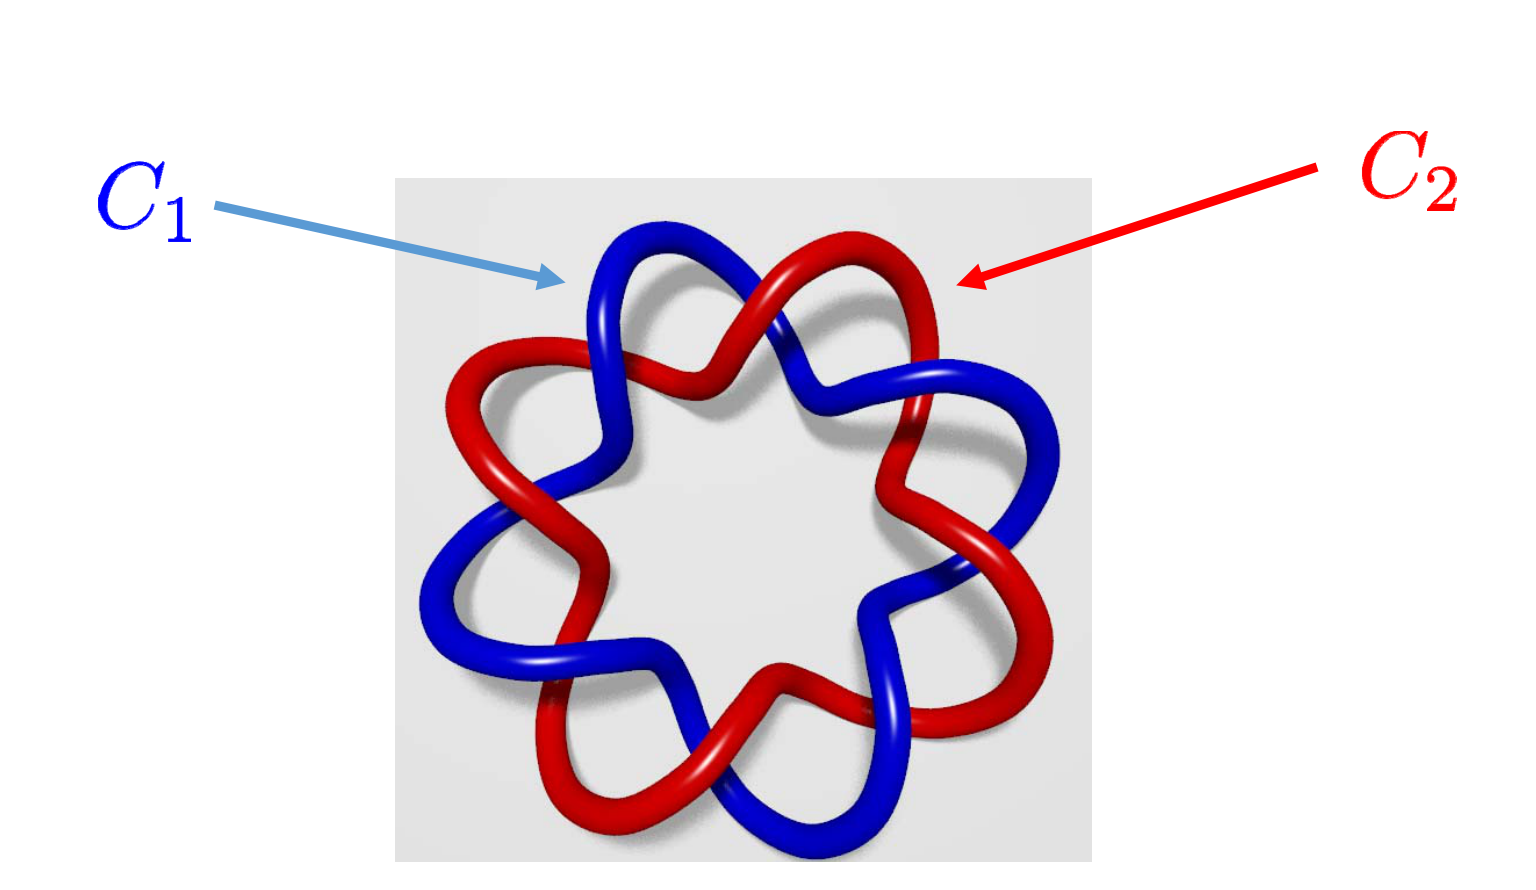
\includegraphics[width=0.55\textwidth]{figures/fig05.png}
  \caption{$\mathbb{R}^3$ 中两条相互链接的曲线 $C_1$ 与 $C_2$。（原文 Fig.~5，第 62 页）}
  \label{fig:5}
\end{figure}

\medskip
\noindent\textbf{评注}：$L(C_1,C_2)$ 的积分公式由 Gauss 于 1833 年发现。它与两个电流圈互感系数的 Neumann 公式有某些相似之处，但实际上相当不同。

我们断言 $L(C,C')$ 实际上是一个整数，它度量 $C$ 与 $C'$ 的链接。在静磁学中，如果我们不担心反转定向的时空变换，可以把 $\vec B$ 看作定义了 $\mathbb{R}^3$ 上的一个 $1$-形式，即 $B=B^idx^i$。类似地，可以把电流 $\vec J$ 看作定义了一个 $2$-形式 $J=\frac{1}{2}\epsilon_{ijk}J^idx^jdx^k$。这里我们用的是 $\mathbb{R}^3$ 中 $1$-形式与 $2$-形式之间的 Hodge 对偶，以及由欧氏度规给出的向量与 $1$-形式的等同。

无论如何，把 $B$ 等同于 $1$-形式、$J$ 等同于 $2$-形式之后，Biot–Savart 定律等价于：

\begin{equation}
  dB=J
  \tag{2.262}
  \label{eq:2.262}
\end{equation}

而所做的功正是 $\int_{C'}B$。

现在取 $I=1$，并令 $D'$ 是张在 $C'$ 上的一个定向圆盘，如图 6 所示。然后我们计算流过 $D'$ 的总电流：

\begin{equation}
  \begin{aligned}
    \oint_{C'}B&=\int_{D'}dB=\int_{D'}J\\
    &=\int_{D'}d\xi^\alpha\wedge d\xi^\beta\,
    \frac{\partial x^m}{\partial\xi^\alpha}\frac{\partial x^n}{\partial\xi^\beta}
    \frac{1}{2}\epsilon_{mnj}\oint_C\frac{dx^j(t)}{dt}\delta^{(3)}\big(\vec x(\xi)-\vec x(t)\big)
  \end{aligned}
  \tag{2.263}
  \label{eq:2.263}
\end{equation}
% [Tutor Note: 从 (2.263) 到「每个横截交点贡献 $\pm1$」省掉了一步：把沿 $C$ 的 $\delta^{(3)}$ 积分与 $\int_{D'}$ 交换次序后，$\int_{D'}d\xi^1d\xi^2\,\delta^{(3)}(\vec x(\xi)-\vec x(t))$ 只在 $D'$ 与 $C$ 横截相交的那些 $\xi$ 处非零，其值为 $1/|n\cdot\dot x(t)|$（$n$ 为 $D'$ 的法向）；再乘上 $\frac{1}{2}\epsilon_{mnj}\frac{\partial x^m}{\partial\xi^\alpha}\frac{\partial x^n}{\partial\xi^\beta}\dot x^j$——即 $\dot x$ 与 $D'$ 两条切向量的混合积——恰好约成 $\pm1$，符号由 $D'$ 的定向（由 $C'$ 诱导）与 $C$ 的定向共同决定。]

\begin{figure}[htbp]
  \centering
  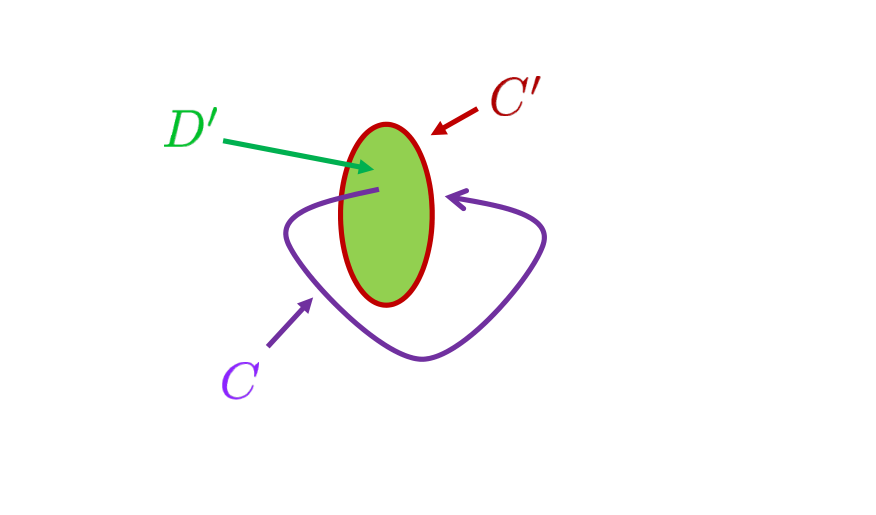
\includegraphics[width=0.42\textwidth]{figures/fig06.png}
  \caption{若用圆盘 $D'$ 填充 $C'$，则可证明 $L(C,C')$ 计数 $C'$ 与 $D'$ 的带符号相交数，因而是一个整数。（原文 Fig.~6，第 63 页）}
  \label{fig:6}
\end{figure}

其中 $\xi^\alpha$ 是 $D'$ 上的一些坐标。容易看出，在最后一个表达式中，$D'$ 与 $C$ 的每个横截\emph{相交}按定向贡献 $\pm1$：$C'$ 的定向在 $D'$ 上诱导出一个定向，而 $C$ 是定向的。这个带定向的相交数就是环绕数的定义之一。由这一解释，$L(C,C')$ 显然在 $D'$ 或 $C$ 或 $C'$ 的连续形变下不变，只要 $C$ 与 $C'$ 不交叉。

既然 $L(C,C')$ 是 $C$ 与 $C'$ 位置的\emph{连续}函数，另一方面它又是\emph{整数}，因此它是一个\emph{拓扑不变量}。注意，如果我们允许 $C$ 与 $C'$ 交叉，这个拓扑不变量就可能改变。当 $C$ 与 $C'$ 交叉时，公式 \eqref{eq:2.261} 变得不良定义，于是这个整数可以跳变。

\medskip
\noindent\textbf{练习}（\emph{拓扑不变性的显式验证}）\quad 证明 $I(C_1,C_2)$ 在 $\vec x_1(t)$ 的小形变下不变，做法是对公式 \eqref{eq:2.261} 作显式变分。

\medskip
\noindent\textbf{练习}\quad 定义 $\mathbb{R}^3-\{0\}$ 上的 $2$-形式

\begin{equation}
  \omega(x):=\frac{1}{8\pi}\frac{\epsilon_{ijk}x^idx^jdx^k}{|x|^3}
  \tag{2.264}
  \label{eq:2.264}
\end{equation}

a.) 证明：当限制到单位球面 $S^2\subset\mathbb{R}^3-\{0\}$ 上时，形式 $\omega$ 限制为体积等于 $1$ 的标准体积形式。

b.) 证明 Gauss 环绕数可以优雅地表示为：

\begin{equation}
  L(C_1,C_2)=\int_{C_1}\int_{C_2}\omega(x_1-x_2)
  \tag{2.265}
  \label{eq:2.265}
\end{equation}

\medskip
% [Tutor Note: 上一题 a.) 与 b.) 之间有一个容易漏掉的因子 2。(2.265) 里要展开 $\omega(x_1-x_2)$，必须用 $d(x_1-x_2)=dx_1-dx_2$ 并把 $dx_1\wedge dx_1=dx_2\wedge dx_2=0$ 用上：$d(x_1-x_2)^j\wedge d(x_1-x_2)^k=-2\,dx_1^j\wedge dx_2^k$，于是 $\omega(x_1-x_2)=-\frac{1}{4\pi}\epsilon_{ijk}(x_1-x_2)^idx_1^jdx_2^k$，与 (2.261) 的被积函数逐项相同（$1/8\pi$ 与 $2$ 一起给出 $1/4\pi$，负号则与 (2.261) 的 $-\frac{1}{4\pi}$ 一致）。若直接把 $d(x_1-x_2)$ 当成 $dx_1$，就会漏掉这个因子 2，并误以为 (2.257)、(2.265) 与 (2.261) 相差一个因子 $-2$。另外这一题里 $I(C_1,C_2)$ 按上下文应为 $L(C_1,C_2)$，原文如此，译文照录。]
